% set 0.5 inch indentation
\setlength{\parindent}{0in}
% set paragraph space = 0 space
\setlength{\parskip}{1.5mm}
% set line space 1.5
\setlength{\baselineskip}{1.6em}

\chapter{INTRODUCTION}
\section{Background}
\acrfull{vl} models have gained significant attention due to their ability to perform zero-shot and transfer learning, achieving high performance across numerous downstream tasks through pre-training with web-scale image-text pairs.
Many \acrshort{vl} models incorporate \acrfull{mlm} as a pre-training task, making it a fundamental approach for training \acrshort{vl} models \cite{albef, mplug, uniter, beit-3}.
Typically, a subset of word tokens is randomly masked at a fixed percentage during training, and the model is tasked with predicting these masked tokens using information from the visual modality.
This masking approach has proven to enhance the alignment between visual and linguistic representations, significantly boosting performance in vision-language tasks.

However, the impact of \acrshort{mlm} on \acrshort{vl} training remains underexplored.
\citeA{mask_object} demonstrated that many of the masked tokens are often stop-words or punctuation, leading the model to rely more on language patterns that do not require visual understanding.
By focusing on masking objects instead, this approach showed improvements in both performance and efficiency compared to random masking \cite{mask_object}.
Another study by \citeA{selective_masking} found that selectively masking infrequent words from the pre-training dataset during continued training enhances model performance on out-of-domain datasets.
Furthermore, \citeA{rf-curriculum-masking} introduced a curriculum masking scheme where a reinforcement learning agent selects masking spans based on cross-model interactions, leading to improved relational understanding with a reduced training dataset.
These works underscore the importance of selecting appropriate tokens for masking.

Despite the widespread adoption of \acrshort{mlm} in \acrshort{vl} training, its effects on model performance and learning dynamics remain underexplored.
\citeA{mask_object} highlighted that many of the randomly masked tokens are often stop-words or punctuation, which encourages the model to rely on linguistic patterns that require minimal visual understanding.
To address this, they proposed masking object-related tokens, which led to notable improvements in model performance and training efficiency compared to random masking \cite{mask_object}.
Similarly, \citeA{selective_masking} demonstrated that selectively masking infrequent words from the pre-training dataset can boost model performance on out-of-domain datasets during continued training.
Additionally, \citeA{rf-curriculum-masking} introduced a curriculum-based masking strategy, where a reinforcement learning agent dynamically selects masking spans based on cross-model interactions. This approach improved the model's relational understanding while reducing the dataset size required for effective training.
These findings collectively emphasize the importance of strategic token selection in \acrshort{mlm} to enhance \acrshort{vl} model learning and efficiency.

In this work, we explore the effects of masking each part-of-speech category by masking each part-of-speech of each image captions as shown in figure \ref{fig:overview}. 
As each part-of-speech contributes uniquely to the meaning of a sentence, for instance, nouns typically represent objects, while verbs describe actions, which often require contextual understanding. 
We hypothesize that masking verbs is the best way to increase the VL model understanding, as verbs in a sentence represent interactions between objects and require the model to rely more on visual information.
By selectively masking different part-of-speech, we can gain insight about how each part-of-speech category affects the alignment between vision and language modalities. 
The experiment is designed to answer the following questions:
\begin{enumerate}
    \item How does selective part-of-speech masking affect the alignment of vision and language modalities?
    \item How does part-of-speech masking change the contribution of the vision and language modalities to the model's output?
    \item How does specific masking impact the performance of vision question answering tasks, particularly in terms of improvements based on the type of question?
\end{enumerate}

\begin{figure}[h]
    \caption{Overall methodology}
    \label{fig:overview}
    Pre-training model with MLM task by masking token based on part-of-speech of the image captions.
    \begin{center}
        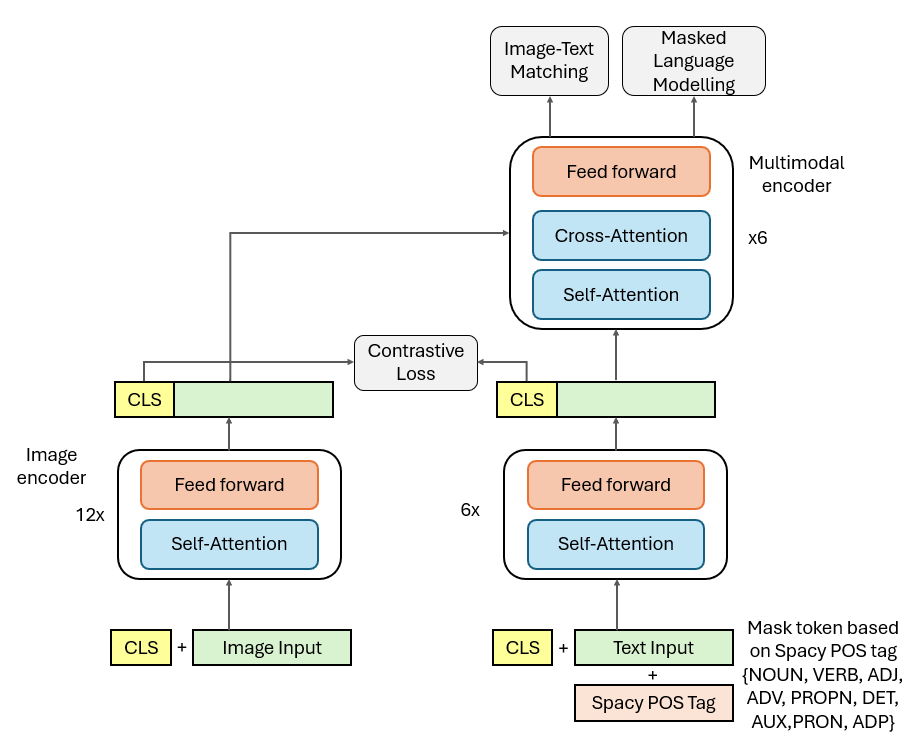
\includegraphics[width=0.6\textwidth]{Images/overview.png}
    \end{center}
    \small
\end{figure}

\section{Objective}
The objectives for our experiment are as listed.
\begin{enumerate}
    \item Pre-trained VL model for the experiment to identify the performance of masking in each part-of-speech.
    \item Benchmarking our method against specialize dataset based on linguistic feature \cite{valse} for better understanding of the masking effect.
    \item Analyze contribution from each modality of vision and language to the prediction output based on MM-Shap \cite{mm-shap}.
\end{enumerate}

\section{Scope}
\begin{enumerate}
    \item The training and testing dataset are both natural image.
    \item The model architecture is cross-attention model due to the ability of cross attention to jointly predicted answer based on another modality.
\end{enumerate}


